\documentclass{standalone}
\usepackage{tikz}
\usetikzlibrary{
  arrows,
  calc,
  decorations.pathmorphing,
  decorations.pathreplacing,
  decorations.markings,
  fadings,
  positioning,
  shapes,
  arrows.meta
}
\pgfdeclareradialshading{glow}{\pgfpoint{0cm}{0cm}}{
  color(0mm)=(white);
  color(5mm)=(white);
  color(9mm)=(black);
  color(10mm)=(black)
}

\begin{tikzfadingfrompicture}[name=glow fading]
  \shade [shading=glow] (0,0) circle (1);
\end{tikzfadingfrompicture}

\ifpdf
% Ensure reproducible output
\pdfinfoomitdate=1
\pdfsuppressptexinfo=-1
\pdftrailerid{}
\fi

\begin{document}

\begin{tikzpicture}
  \node at (-4.8, 1.5) {
\includegraphics[width=3.0cm]{apparatus}};
  \node at (-6.4, 1.8) {\footnotesize (\textbf{A})};
  \node at (-4.8, -0.7) {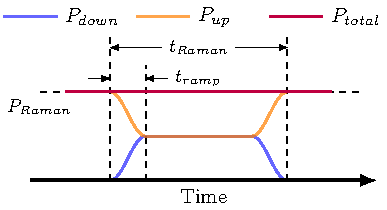
\includegraphics[width=4.5cm]{sequence}};
  \node at (-6.7, -1.35) {\footnotesize (\textbf{B})};
  \node at (0, 0) {\includegraphics[width=5cm]{../../experiments/nacs_202003/imgs/fit_20200326_005204_raman_3322_2_damop_f_text.pdf}};
  \node at (-1.4, -1.1) {\footnotesize (\textbf{C})};
  \node at (5, 0) {\includegraphics[width=5cm]{../../experiments/nacs_202007/imgs/fit_20200703_201618_raman15_3322_2_postdoc_t.pdf}};
  \node at (3.5, -1.1) {\footnotesize (\textbf{D})};
\end{tikzpicture}

\end{document}
